% Options for packages loaded elsewhere
\PassOptionsToPackage{unicode}{hyperref}
\PassOptionsToPackage{hyphens}{url}
\documentclass[
]{article}
\usepackage{xcolor}
\usepackage{amsmath,amssymb}
\setcounter{secnumdepth}{-\maxdimen} % remove section numbering
\usepackage{iftex}
\ifPDFTeX
  \usepackage[T1]{fontenc}
  \usepackage[utf8]{inputenc}
  \usepackage{textcomp} % provide euro and other symbols
\else % if luatex or xetex
  \usepackage{unicode-math} % this also loads fontspec
  \defaultfontfeatures{Scale=MatchLowercase}
  \defaultfontfeatures[\rmfamily]{Ligatures=TeX,Scale=1}
\fi
\usepackage{lmodern}
\ifPDFTeX\else
  % xetex/luatex font selection
\fi
% Use upquote if available, for straight quotes in verbatim environments
\IfFileExists{upquote.sty}{\usepackage{upquote}}{}
\IfFileExists{microtype.sty}{% use microtype if available
  \usepackage[]{microtype}
  \UseMicrotypeSet[protrusion]{basicmath} % disable protrusion for tt fonts
}{}
\makeatletter
\@ifundefined{KOMAClassName}{% if non-KOMA class
  \IfFileExists{parskip.sty}{%
    \usepackage{parskip}
  }{% else
    \setlength{\parindent}{0pt}
    \setlength{\parskip}{6pt plus 2pt minus 1pt}}
}{% if KOMA class
  \KOMAoptions{parskip=half}}
\makeatother
\usepackage{longtable,booktabs,array}
\usepackage{calc} % for calculating minipage widths
% Correct order of tables after \paragraph or \subparagraph
\usepackage{etoolbox}
\makeatletter
\patchcmd\longtable{\par}{\if@noskipsec\mbox{}\fi\par}{}{}
\makeatother
% Allow footnotes in longtable head/foot
\IfFileExists{footnotehyper.sty}{\usepackage{footnotehyper}}{\usepackage{footnote}}
\makesavenoteenv{longtable}
\usepackage{graphicx}
\makeatletter
\newsavebox\pandoc@box
\newcommand*\pandocbounded[1]{% scales image to fit in text height/width
  \sbox\pandoc@box{#1}%
  \Gscale@div\@tempa{\textheight}{\dimexpr\ht\pandoc@box+\dp\pandoc@box\relax}%
  \Gscale@div\@tempb{\linewidth}{\wd\pandoc@box}%
  \ifdim\@tempb\p@<\@tempa\p@\let\@tempa\@tempb\fi% select the smaller of both
  \ifdim\@tempa\p@<\p@\scalebox{\@tempa}{\usebox\pandoc@box}%
  \else\usebox{\pandoc@box}%
  \fi%
}
% Set default figure placement to htbp
\def\fps@figure{p}
\makeatother
\setlength{\emergencystretch}{3em} % prevent overfull lines
\let\latexunderscore\_
\renewcommand{\_}{\latexunderscore\hspace{0pt}} % allow line breaks after escaped underscores
\providecommand{\tightlist}{%
  \setlength{\itemsep}{0pt}\setlength{\parskip}{0pt}}
\usepackage{bookmark}
\IfFileExists{xurl.sty}{\usepackage{xurl}}{} % add URL line breaks if available
\urlstyle{same}
\hypersetup{
  hidelinks,
  pdfcreator={LaTeX via pandoc}}

\author{}
\date{}

\begin{document}

\section{Weekly Report}\label{weekly-report}

\subsection{What I Worked On}\label{what-i-worked-on}

\subsubsection{Profiling}\label{profiling}

\paragraph{ABINIT}\label{abinit}

\begin{itemize}
\tightlist
\item
  \textbf{Path:}
  \texttt{abinit/v2/fullPEAK-scaling-07102026-152428/timing\_summary.csv}
\end{itemize}

\begin{longtable}[]{@{}
  >{\raggedright\arraybackslash}p{(\linewidth - 14\tabcolsep) * \real{0.2800}}
  >{\raggedright\arraybackslash}p{(\linewidth - 14\tabcolsep) * \real{0.1028}}
  >{\raggedright\arraybackslash}p{(\linewidth - 14\tabcolsep) * \real{0.1028}}
  >{\raggedright\arraybackslash}p{(\linewidth - 14\tabcolsep) * \real{0.1028}}
  >{\raggedright\arraybackslash}p{(\linewidth - 14\tabcolsep) * \real{0.1028}}
  >{\raggedright\arraybackslash}p{(\linewidth - 14\tabcolsep) * \real{0.1028}}
  >{\raggedright\arraybackslash}p{(\linewidth - 14\tabcolsep) * \real{0.1028}}
  >{\raggedright\arraybackslash}p{(\linewidth - 14\tabcolsep) * \real{0.1028}}@{}}
\toprule\noalign{}
\begin{minipage}[b]{\linewidth}\raggedright
Job Name
\end{minipage} & \begin{minipage}[b]{\linewidth}\raggedright
Config
\end{minipage} & \begin{minipage}[b]{\linewidth}\raggedright
Nodes
\end{minipage} & \begin{minipage}[b]{\linewidth}\raggedright
Tasks
\end{minipage} & \begin{minipage}[b]{\linewidth}\raggedright
PEAK?
\end{minipage} & \begin{minipage}[b]{\linewidth}\raggedright
Elapsed (s)
\end{minipage} & \begin{minipage}[b]{\linewidth}\raggedright
Exit Code
\end{minipage} & \begin{minipage}[b]{\linewidth}\raggedright
Job ID
\end{minipage} \\
\midrule\noalign{}
\endhead
\bottomrule\noalign{}
\endlastfoot
\texttt{abinit\_test\_n1\_nopeak} & \texttt{n1\_nopeak} & 1 & 1 & No &
\textbf{119} & 0 & 3294914 \\
\texttt{abinit\_test\_n24\_nopeak} & \texttt{n24\_nopeak} & 1 & 24 & No
& \textbf{10} & 0 & 3294915 \\
\texttt{abinit\_test\_n48\_nopeak} & \texttt{n48\_nopeak} & 1 & 48 & No
& \textbf{8} & 0 & 3294916 \\
\texttt{abinit\_test\_N2\_nopeak} & \texttt{N2\_nopeak} & 2 & 96 & No &
\textbf{6} & 0 & 3294917 \\
\texttt{abinit\_test\_N8\_nopeak} & \texttt{N8\_nopeak} & 8 & 384 & No &
\textbf{6} & 0 & 3294918 \\
\texttt{abinit\_test\_N16\_nopeak} & \texttt{N16\_nopeak} & 16 & 768 &
No & \textbf{9} & 0 & 3294919 \\
\texttt{abinit\_test\_n1\_peak} & \texttt{n1\_peak} & 1 & 1 & Yes &
\textbf{126} & 0 & 3294920 \\
\end{longtable}

\begin{longtable}[]{@{}
  >{\raggedright\arraybackslash}p{(\linewidth - 8\tabcolsep) * \real{0.2000}}
  >{\raggedright\arraybackslash}p{(\linewidth - 8\tabcolsep) * \real{0.2000}}
  >{\raggedright\arraybackslash}p{(\linewidth - 8\tabcolsep) * \real{0.2000}}
  >{\raggedright\arraybackslash}p{(\linewidth - 8\tabcolsep) * \real{0.2000}}
  >{\raggedright\arraybackslash}p{(\linewidth - 8\tabcolsep) * \real{0.2000}}@{}}
\toprule\noalign{}
\begin{minipage}[b]{\linewidth}\raggedright
Function
\end{minipage} & \begin{minipage}[b]{\linewidth}\raggedright
Calls
\end{minipage} & \begin{minipage}[b]{\linewidth}\raggedright
Total Time (s)
\end{minipage} & \begin{minipage}[b]{\linewidth}\raggedright
Avg Time / Call (ms)
\end{minipage} & \begin{minipage}[b]{\linewidth}\raggedright
PEAK Overhead (s)
\end{minipage} \\
\midrule\noalign{}
\endhead
\bottomrule\noalign{}
\endlastfoot
\texttt{zgemm\_} & 207,990 & \textbf{4.7613} & 0.0229 & 0.4258 \\
\texttt{ddot\_} & 216,544 & \textbf{0.6383} & 0.0029 & 0.4433 \\
\texttt{zcopy\_} & 131,022 & \textbf{0.6081} & 0.0046 & 0.2682 \\
\texttt{dznrm2\_} & 116,280 & \textbf{0.5958} & 0.0051 & 0.2380 \\
\texttt{zdotc\_} & 51,588 & \textbf{0.1846} & 0.0036 & 0.1056 \\
\end{longtable}

\begin{figure}
\centering
\pandocbounded{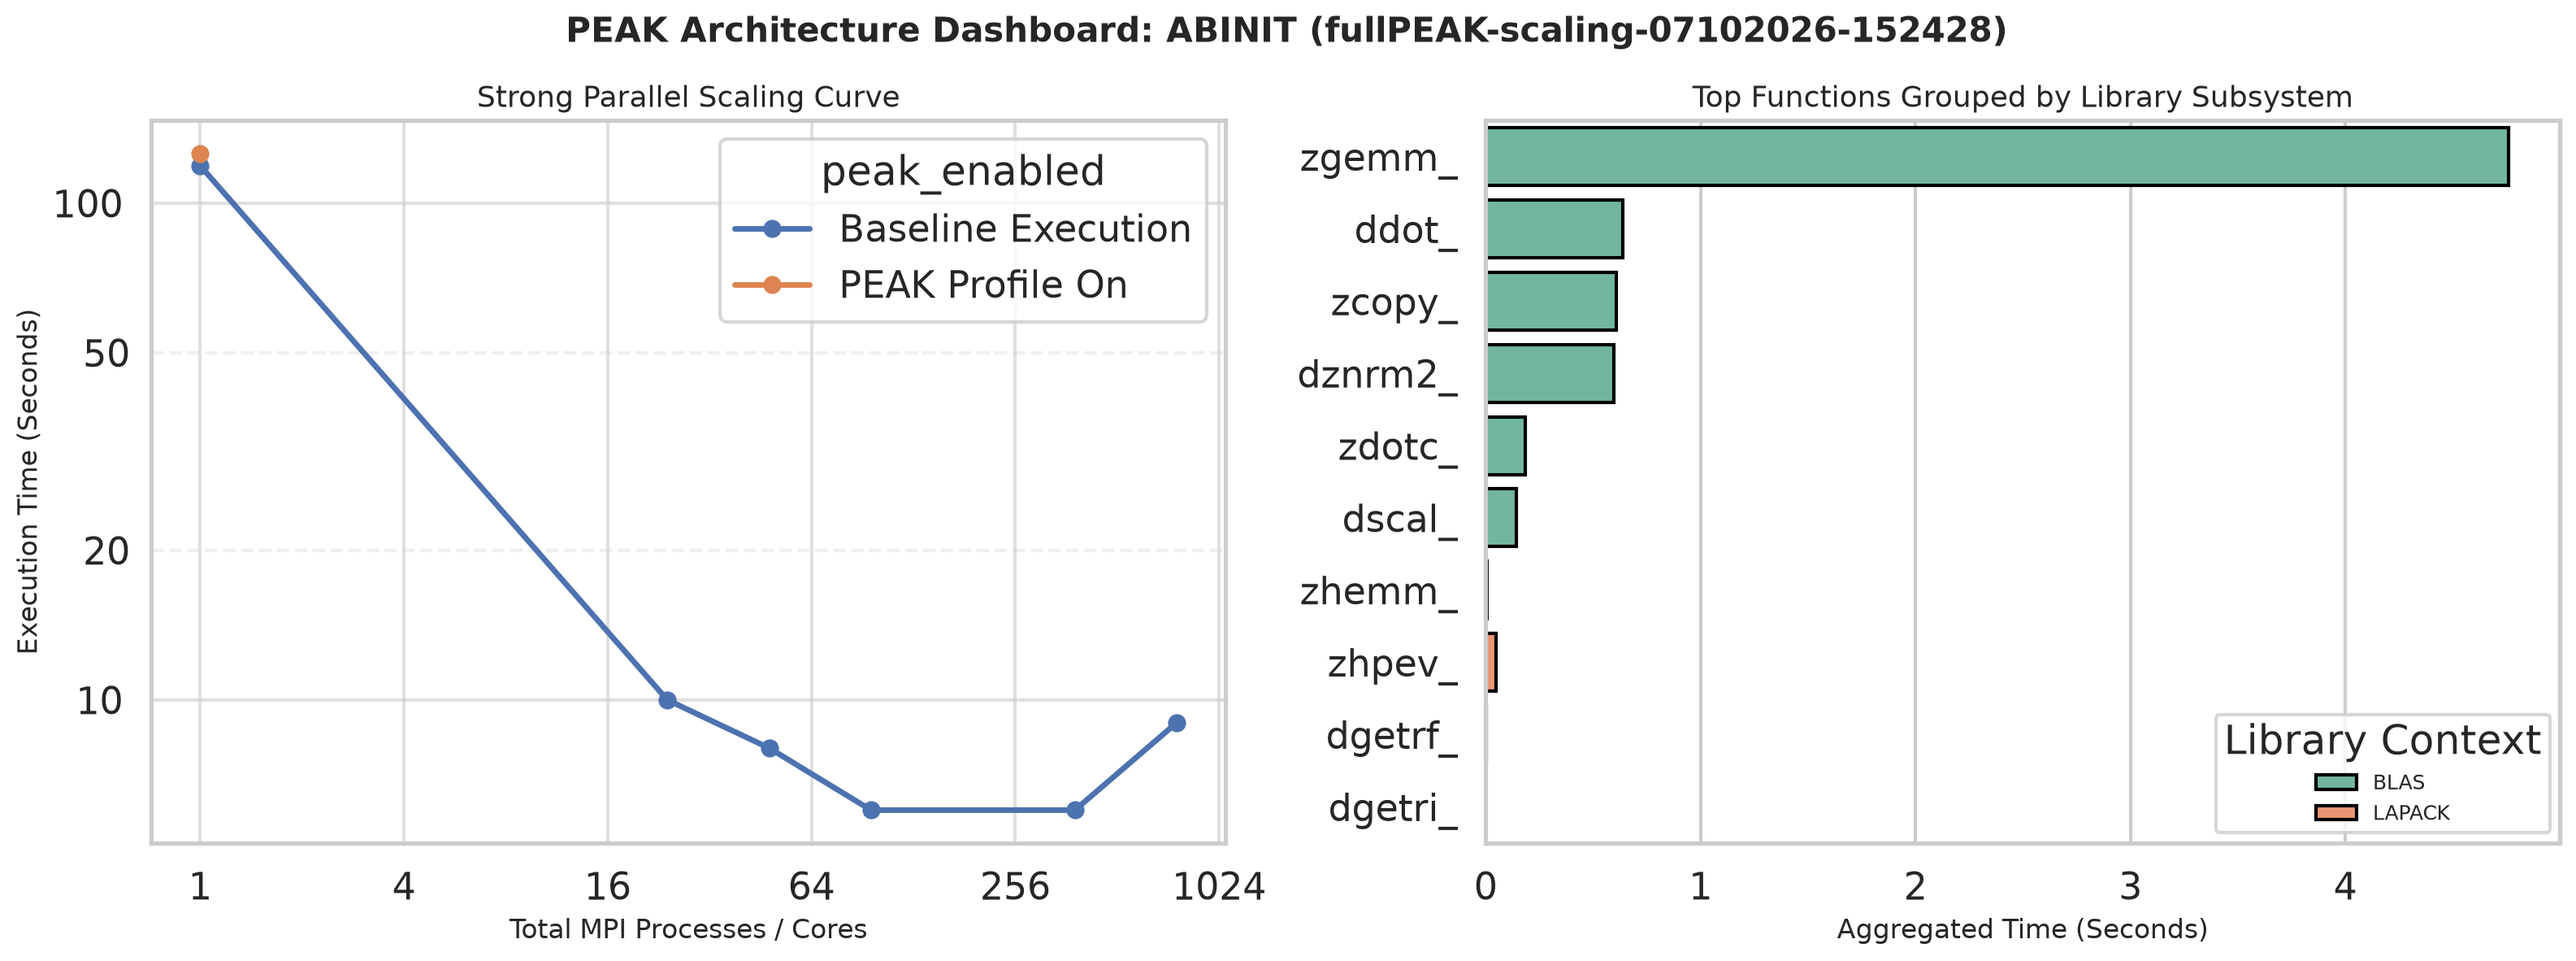
\includegraphics[keepaspectratio]{../plots/abinit_fullPEAK-scaling-07102026-152428_dashboard.png}}
\caption{plot}
\end{figure}

\subparagraph{Takeaway}\label{takeaway}

\begin{itemize}
\tightlist
\item
  ABINIT effectively scaled from 1 to 96 tasks but performs worse when
  scaled further on this test case.
\item
  As I understand it, the decrease in speed up is most likely due to
  inter-node communication overhead.
\end{itemize}

\paragraph{Quantum Espresso}\label{quantum-espresso}

\begin{itemize}
\tightlist
\item
  \textbf{Path:}
  \texttt{qe/fftw\_test-scaling-07142026-092819/timing\_summary.csv}
\end{itemize}

\begin{longtable}[]{@{}
  >{\raggedright\arraybackslash}p{(\linewidth - 14\tabcolsep) * \real{0.2800}}
  >{\raggedright\arraybackslash}p{(\linewidth - 14\tabcolsep) * \real{0.1028}}
  >{\raggedright\arraybackslash}p{(\linewidth - 14\tabcolsep) * \real{0.1028}}
  >{\raggedright\arraybackslash}p{(\linewidth - 14\tabcolsep) * \real{0.1028}}
  >{\raggedright\arraybackslash}p{(\linewidth - 14\tabcolsep) * \real{0.1028}}
  >{\raggedright\arraybackslash}p{(\linewidth - 14\tabcolsep) * \real{0.1028}}
  >{\raggedright\arraybackslash}p{(\linewidth - 14\tabcolsep) * \real{0.1028}}
  >{\raggedright\arraybackslash}p{(\linewidth - 14\tabcolsep) * \real{0.1028}}@{}}
\toprule\noalign{}
\begin{minipage}[b]{\linewidth}\raggedright
Job Name
\end{minipage} & \begin{minipage}[b]{\linewidth}\raggedright
Config
\end{minipage} & \begin{minipage}[b]{\linewidth}\raggedright
Nodes
\end{minipage} & \begin{minipage}[b]{\linewidth}\raggedright
Tasks
\end{minipage} & \begin{minipage}[b]{\linewidth}\raggedright
PEAK?
\end{minipage} & \begin{minipage}[b]{\linewidth}\raggedright
Elapsed (s)
\end{minipage} & \begin{minipage}[b]{\linewidth}\raggedright
Exit Code
\end{minipage} & \begin{minipage}[b]{\linewidth}\raggedright
Job ID
\end{minipage} \\
\midrule\noalign{}
\endhead
\bottomrule\noalign{}
\endlastfoot
\texttt{qe\_tc\_n1\_nopeak} & \texttt{n1\_nopeak} & 1 & 1 & No &
\textbf{636} & 0 & 3306688 \\
\texttt{qe\_tc\_n24\_nopeak} & \texttt{n24\_nopeak} & 1 & 24 & No &
\textbf{63} & 0 & 3306689 \\
\texttt{qe\_tc\_n48\_nopeak} & \texttt{n48\_nopeak} & 1 & 48 & No &
\textbf{34} & 0 & 3306690 \\
\texttt{qe\_tc\_N2\_nopeak} & \texttt{N2\_nopeak} & 2 & 96 & No &
\textbf{28} & 0 & 3306691 \\
\texttt{qe\_tc\_N8\_nopeak} & \texttt{N8\_nopeak} & 8 & 384 & No &
\textbf{20} & 0 & 3306692 \\
\texttt{qe\_tc\_N16\_nopeak} & \texttt{N16\_nopeak} & 16 & 768 & No &
\textbf{27} & 0 & 3306693 \\
\texttt{qe\_tc\_n1\_peak} & \texttt{n1\_peak} & 1 & 1 & Yes &
\textbf{638} & 0 & 3306694 \\
\end{longtable}

\begin{longtable}[]{@{}
  >{\raggedright\arraybackslash}p{(\linewidth - 8\tabcolsep) * \real{0.2000}}
  >{\raggedright\arraybackslash}p{(\linewidth - 8\tabcolsep) * \real{0.2000}}
  >{\raggedright\arraybackslash}p{(\linewidth - 8\tabcolsep) * \real{0.2000}}
  >{\raggedright\arraybackslash}p{(\linewidth - 8\tabcolsep) * \real{0.2000}}
  >{\raggedright\arraybackslash}p{(\linewidth - 8\tabcolsep) * \real{0.2000}}@{}}
\toprule\noalign{}
\begin{minipage}[b]{\linewidth}\raggedright
Function
\end{minipage} & \begin{minipage}[b]{\linewidth}\raggedright
Calls
\end{minipage} & \begin{minipage}[b]{\linewidth}\raggedright
Total Time (s)
\end{minipage} & \begin{minipage}[b]{\linewidth}\raggedright
Avg Time / Call (ms)
\end{minipage} & \begin{minipage}[b]{\linewidth}\raggedright
PEAK Overhead (s)
\end{minipage} \\
\midrule\noalign{}
\endhead
\bottomrule\noalign{}
\endlastfoot
\texttt{zgemm\_} & 144,849 & \textbf{166.6082} & 1.1502 & 0.2227 \\
\texttt{zhegvx\_} & 5,561 & \textbf{8.3896} & 1.5087 & 0.0085 \\
\texttt{zgemv\_} & 1,184 & \textbf{3.7863} & 3.1979 & 0.0018 \\
\texttt{ddot\_} & 57,984 & \textbf{0.3923} & 0.0068 & 0.0891 \\
\texttt{dcopy\_} & 1,926 & \textbf{0.3207} & 0.1665 & 0.0030 \\
\end{longtable}

\begin{figure}
\centering
\pandocbounded{
\includegraphics[keepaspectratio]{../plots/qe_fftw_test-scaling-07142026-092819_dashboard.png}}
\caption{plot}
\end{figure}

\subparagraph{Takeaway}\label{takeaway-1}

\begin{itemize}
\tightlist
\item
  Similiar story to ABINIT
\end{itemize}

\paragraph{DFTB+}\label{dftb}

\begin{itemize}
\tightlist
\item
  \textbf{Path:}
  \texttt{dftb/new\_gen-scaling-07132026-145728/timing\_summary.csv}
\end{itemize}

\begin{longtable}[]{@{}
  >{\raggedright\arraybackslash}p{(\linewidth - 14\tabcolsep) * \real{0.2800}}
  >{\raggedright\arraybackslash}p{(\linewidth - 14\tabcolsep) * \real{0.1028}}
  >{\raggedright\arraybackslash}p{(\linewidth - 14\tabcolsep) * \real{0.1028}}
  >{\raggedright\arraybackslash}p{(\linewidth - 14\tabcolsep) * \real{0.1028}}
  >{\raggedright\arraybackslash}p{(\linewidth - 14\tabcolsep) * \real{0.1028}}
  >{\raggedright\arraybackslash}p{(\linewidth - 14\tabcolsep) * \real{0.1028}}
  >{\raggedright\arraybackslash}p{(\linewidth - 14\tabcolsep) * \real{0.1028}}
  >{\raggedright\arraybackslash}p{(\linewidth - 14\tabcolsep) * \real{0.1028}}@{}}
\toprule\noalign{}
\begin{minipage}[b]{\linewidth}\raggedright
Job Name
\end{minipage} & \begin{minipage}[b]{\linewidth}\raggedright
Config
\end{minipage} & \begin{minipage}[b]{\linewidth}\raggedright
Nodes
\end{minipage} & \begin{minipage}[b]{\linewidth}\raggedright
Tasks
\end{minipage} & \begin{minipage}[b]{\linewidth}\raggedright
PEAK?
\end{minipage} & \begin{minipage}[b]{\linewidth}\raggedright
Elapsed (s)
\end{minipage} & \begin{minipage}[b]{\linewidth}\raggedright
Exit Code
\end{minipage} & \begin{minipage}[b]{\linewidth}\raggedright
Job ID
\end{minipage} \\
\midrule\noalign{}
\endhead
\bottomrule\noalign{}
\endlastfoot
\texttt{dftb\_spinlock\_n1\_nopeak} & \texttt{n1\_nopeak} & 1 & 1 & No &
\textbf{120} & 0 & 3303873 \\
\texttt{dftb\_spinlock\_n24\_nopeak} & \texttt{n24\_nopeak} & 1 & 24 &
No & \textbf{144} & 0 & 3303874 \\
\texttt{dftb\_spinlock\_n48\_nopeak} & \texttt{n48\_nopeak} & 1 & 48 &
No & \textbf{220} & 0 & 3303875 \\
\texttt{dftb\_spinlock\_n1\_peak} & \texttt{n1\_peak} & 1 & 1 & Yes &
\textbf{121} & 0 & 3303879 \\
\texttt{dftb\_spinlock\_N2\_nopeak} & \texttt{N2\_nopeak} & 2 & 96 & No
& \textbf{2} & 1 & 3303876 \\
\texttt{dftb\_spinlock\_N8\_nopeak} & \texttt{N8\_nopeak} & 8 & 384 & No
& \textbf{3} & 1 & 3303877 \\
\texttt{dftb\_spinlock\_N16\_nopeak} & \texttt{N16\_nopeak} & 16 & 768 &
No & \textbf{3} & 1 & 3303878 \\
\end{longtable}

\begin{longtable}[]{@{}
  >{\raggedright\arraybackslash}p{(\linewidth - 8\tabcolsep) * \real{0.2000}}
  >{\raggedright\arraybackslash}p{(\linewidth - 8\tabcolsep) * \real{0.2000}}
  >{\raggedright\arraybackslash}p{(\linewidth - 8\tabcolsep) * \real{0.2000}}
  >{\raggedright\arraybackslash}p{(\linewidth - 8\tabcolsep) * \real{0.2000}}
  >{\raggedright\arraybackslash}p{(\linewidth - 8\tabcolsep) * \real{0.2000}}@{}}
\toprule\noalign{}
\begin{minipage}[b]{\linewidth}\raggedright
Function
\end{minipage} & \begin{minipage}[b]{\linewidth}\raggedright
Calls
\end{minipage} & \begin{minipage}[b]{\linewidth}\raggedright
Total Time (s)
\end{minipage} & \begin{minipage}[b]{\linewidth}\raggedright
Avg Time / Call (s)
\end{minipage} & \begin{minipage}[b]{\linewidth}\raggedright
PEAK Overhead (s)
\end{minipage} \\
\midrule\noalign{}
\endhead
\bottomrule\noalign{}
\endlastfoot
\texttt{dsyev\_} & 4 & \textbf{94.1030} & 23.5258 & 0.0000 \\
\texttt{dgemm\_} & 442 & \textbf{10.5098} & 0.0238 & 0.0007 \\
\texttt{dsymm\_} & 4 & \textbf{10.0370} & 2.5092 & 0.0000 \\
\texttt{dlarrv\_} & 4 & \textbf{0.1037} & 0.0259 & 0.0000 \\
\texttt{dcopy\_} & 34,760 & \textbf{0.0280} & 0.0008 & 0.0541 \\
\end{longtable}

\begin{figure}
\centering
\pandocbounded{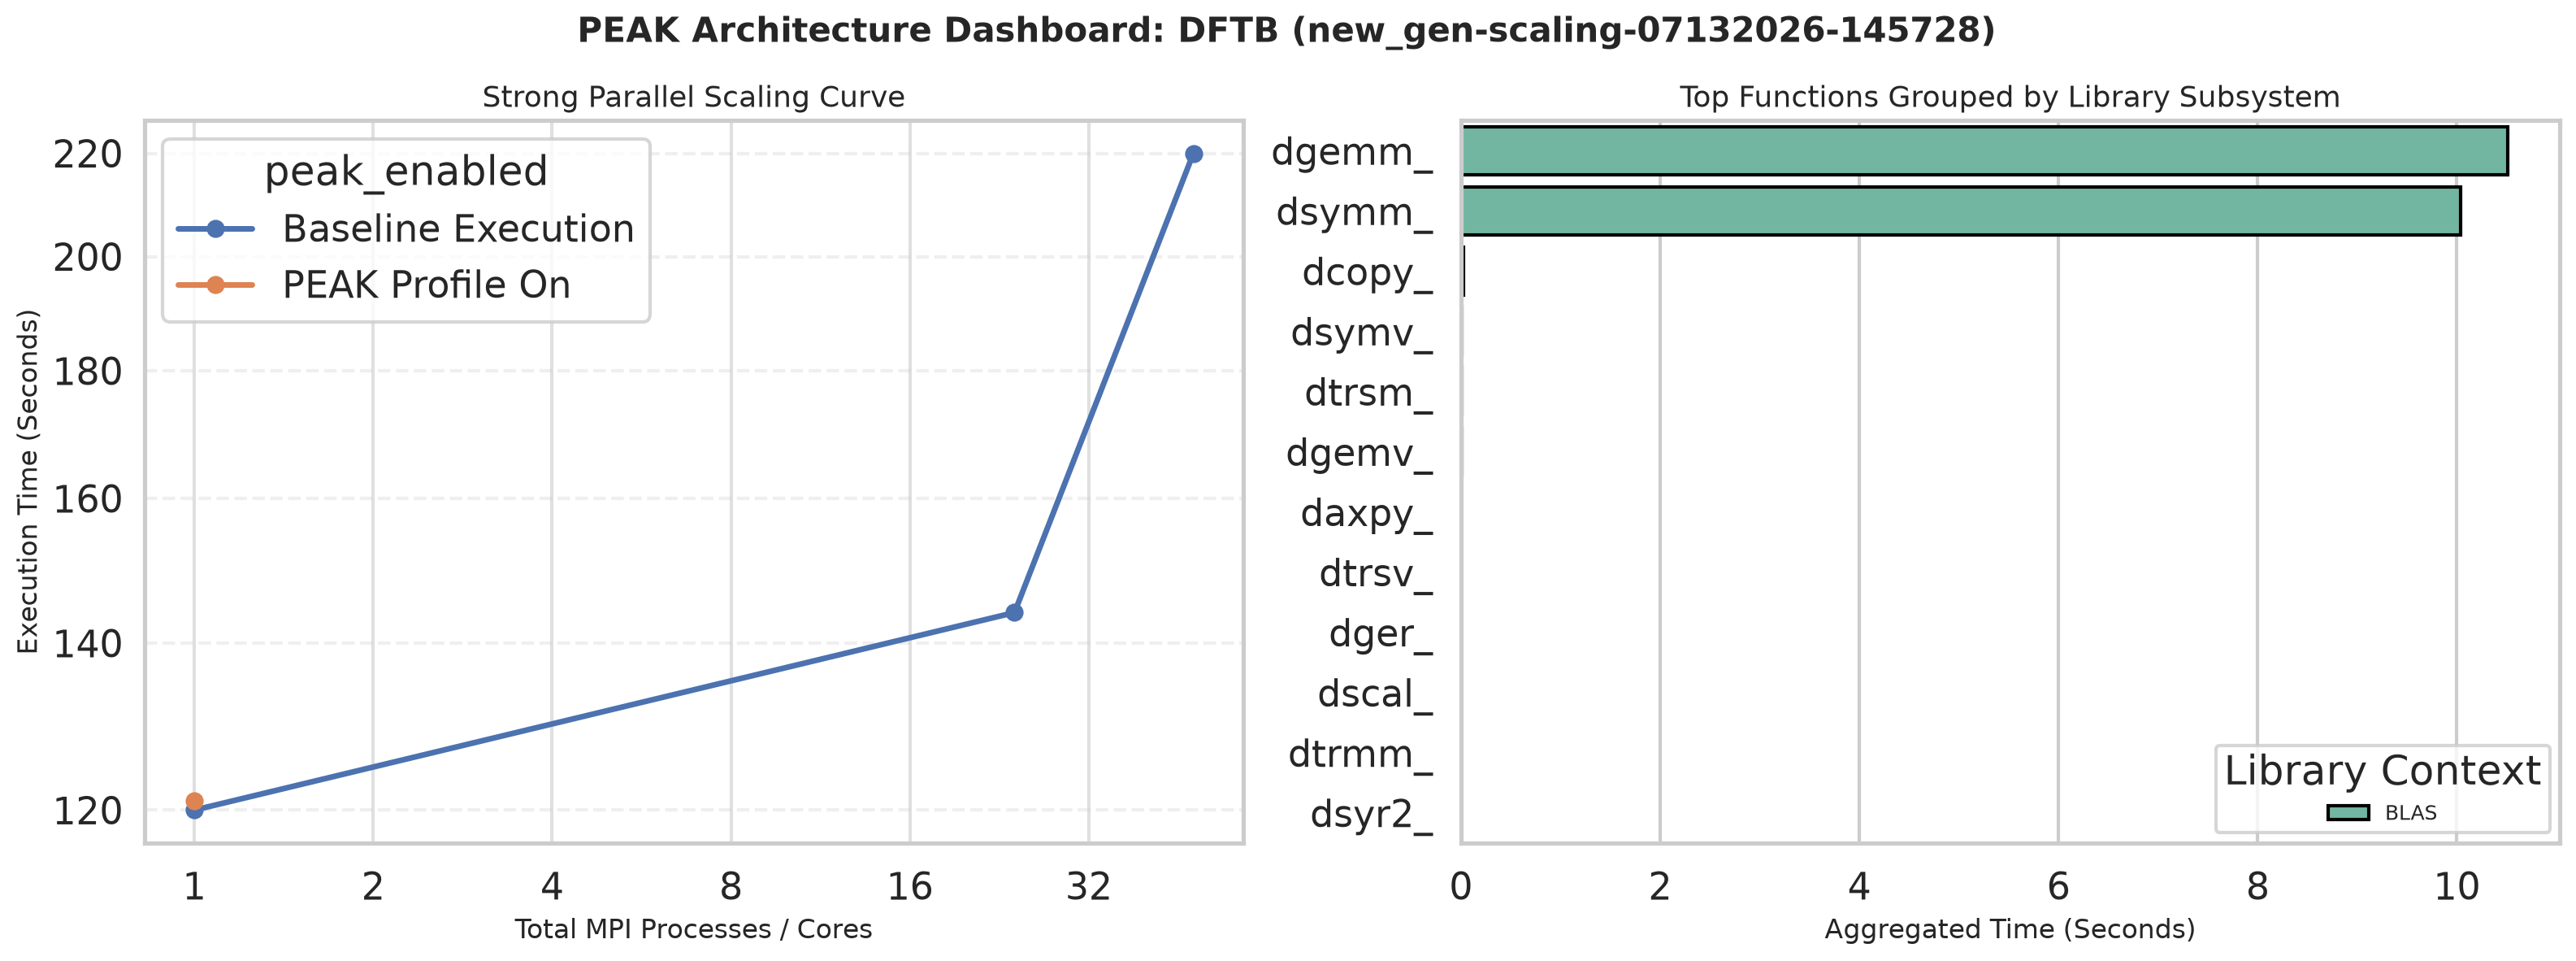
\includegraphics[keepaspectratio]{../plots/dftb_new_gen-scaling-07132026-145728_dashboard.png}}
\caption{plot}
\end{figure}

\subparagraph{Takeaway}\label{takeaway-2}

\begin{itemize}
\tightlist
\item
  DFTB+ seemingly performed worse as it scaled on this test case, even
  crashing on multi-node configurations.
\item
  Im going to look into this one more as it doesn't make sense to me.
\end{itemize}

\paragraph{LAMMPS}\label{lammps}

\begin{itemize}
\tightlist
\item
  \textbf{Path:}
  \texttt{lammps/5-scaling-07132026-225745/timing\_summary.csv}
\end{itemize}

\begin{longtable}[]{@{}
  >{\raggedright\arraybackslash}p{(\linewidth - 14\tabcolsep) * \real{0.2800}}
  >{\raggedright\arraybackslash}p{(\linewidth - 14\tabcolsep) * \real{0.1028}}
  >{\raggedright\arraybackslash}p{(\linewidth - 14\tabcolsep) * \real{0.1028}}
  >{\raggedright\arraybackslash}p{(\linewidth - 14\tabcolsep) * \real{0.1028}}
  >{\raggedright\arraybackslash}p{(\linewidth - 14\tabcolsep) * \real{0.1028}}
  >{\raggedright\arraybackslash}p{(\linewidth - 14\tabcolsep) * \real{0.1028}}
  >{\raggedright\arraybackslash}p{(\linewidth - 14\tabcolsep) * \real{0.1028}}
  >{\raggedright\arraybackslash}p{(\linewidth - 14\tabcolsep) * \real{0.1028}}@{}}
\toprule\noalign{}
\begin{minipage}[b]{\linewidth}\raggedright
Job Name
\end{minipage} & \begin{minipage}[b]{\linewidth}\raggedright
Config
\end{minipage} & \begin{minipage}[b]{\linewidth}\raggedright
Nodes
\end{minipage} & \begin{minipage}[b]{\linewidth}\raggedright
Tasks
\end{minipage} & \begin{minipage}[b]{\linewidth}\raggedright
PEAK?
\end{minipage} & \begin{minipage}[b]{\linewidth}\raggedright
Elapsed (s)
\end{minipage} & \begin{minipage}[b]{\linewidth}\raggedright
Exit Code
\end{minipage} & \begin{minipage}[b]{\linewidth}\raggedright
Job ID
\end{minipage} \\
\midrule\noalign{}
\endhead
\bottomrule\noalign{}
\endlastfoot
\texttt{lammps\_rhodo\_n1\_nopeak} & \texttt{n1\_nopeak} & 1 & 1 & No &
\textbf{32} & 0 & 3305579 \\
\texttt{lammps\_rhodo\_n24\_nopeak} & \texttt{n24\_nopeak} & 1 & 24 & No
& \textbf{4} & 0 & 3305580 \\
\texttt{lammps\_rhodo\_n48\_nopeak} & \texttt{n48\_nopeak} & 1 & 48 & No
& \textbf{4} & 0 & 3305581 \\
\texttt{lammps\_rhodo\_N2\_nopeak} & \texttt{N2\_nopeak} & 2 & 96 & No &
\textbf{4} & 0 & 3305582 \\
\texttt{lammps\_rhodo\_N8\_nopeak} & \texttt{N8\_nopeak} & 8 & 384 & No
& \textbf{4} & 0 & 3305583 \\
\texttt{lammps\_rhodo\_N16\_nopeak} & \texttt{N16\_nopeak} & 16 & 768 &
No & \textbf{8} & 255 & 3305584 \\
\texttt{lammps\_rhodo\_n1\_peak} & \texttt{n1\_peak} & 1 & 1 & Yes &
\textbf{32} & 0 & 3305585 \\
\end{longtable}

\begin{quote}
LAMMPS did not yield any PEAK hits on both module and build script
versions.
\end{quote}

\begin{figure}
\centering
\pandocbounded{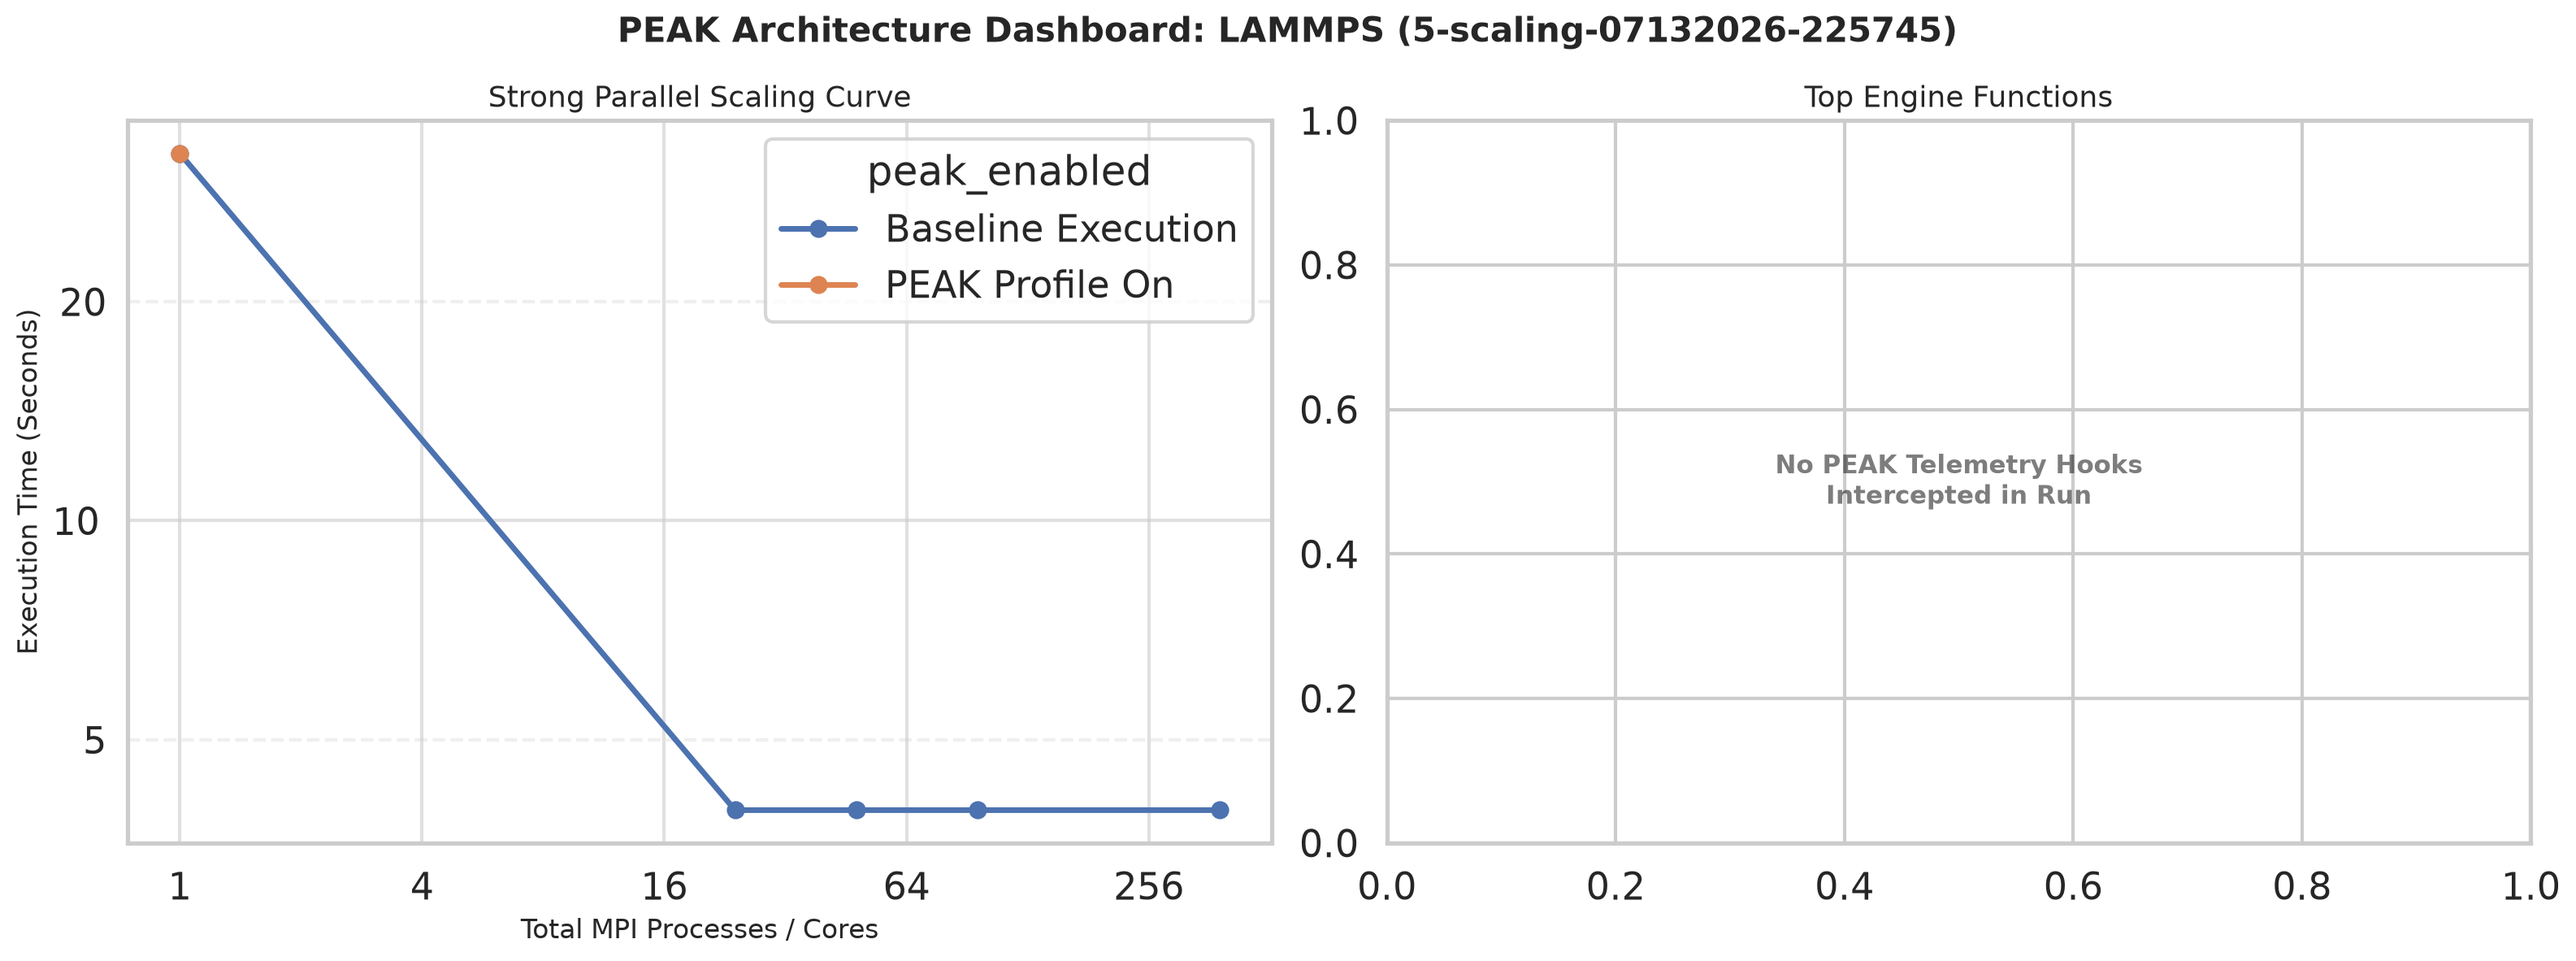
\includegraphics[keepaspectratio]{../plots/lammps_5-scaling-07132026-225745_dashboard.png}}
\caption{plot}
\end{figure}

\subparagraph{Takeaway}\label{takeaway-3}

\begin{itemize}
\tightlist
\item
  LAMMPS scaled great, but seemingly limitted itself after an upper
  limit.
\item
  As I understand it, this limit is based on the input and more complex
  input files will scale better.
\end{itemize}

\paragraph{GROMACS}\label{gromacs}

\begin{itemize}
\tightlist
\item
  \textbf{Path:}
  \texttt{gromacs/2-scaling-07102026-221528/timing\_summary.csv}
\end{itemize}

\begin{longtable}[]{@{}
  >{\raggedright\arraybackslash}p{(\linewidth - 14\tabcolsep) * \real{0.2800}}
  >{\raggedright\arraybackslash}p{(\linewidth - 14\tabcolsep) * \real{0.1028}}
  >{\raggedright\arraybackslash}p{(\linewidth - 14\tabcolsep) * \real{0.1028}}
  >{\raggedright\arraybackslash}p{(\linewidth - 14\tabcolsep) * \real{0.1028}}
  >{\raggedright\arraybackslash}p{(\linewidth - 14\tabcolsep) * \real{0.1028}}
  >{\raggedright\arraybackslash}p{(\linewidth - 14\tabcolsep) * \real{0.1028}}
  >{\raggedright\arraybackslash}p{(\linewidth - 14\tabcolsep) * \real{0.1028}}
  >{\raggedright\arraybackslash}p{(\linewidth - 14\tabcolsep) * \real{0.1028}}@{}}
\toprule\noalign{}
\begin{minipage}[b]{\linewidth}\raggedright
Job Name
\end{minipage} & \begin{minipage}[b]{\linewidth}\raggedright
Config
\end{minipage} & \begin{minipage}[b]{\linewidth}\raggedright
Nodes
\end{minipage} & \begin{minipage}[b]{\linewidth}\raggedright
Tasks
\end{minipage} & \begin{minipage}[b]{\linewidth}\raggedright
PEAK?
\end{minipage} & \begin{minipage}[b]{\linewidth}\raggedright
Elapsed (s)
\end{minipage} & \begin{minipage}[b]{\linewidth}\raggedright
Exit Code
\end{minipage} & \begin{minipage}[b]{\linewidth}\raggedright
Job ID
\end{minipage} \\
\midrule\noalign{}
\endhead
\bottomrule\noalign{}
\endlastfoot
\texttt{gromacs\_benchMEM\_n24\_nopeak} & \texttt{n24\_nopeak} & 1 & 24
& No & \textbf{213} & 0 & 3295859 \\
\texttt{gromacs\_benchMEM\_n48\_nopeak} & \texttt{n48\_nopeak} & 1 & 48
& No & \textbf{125} & 0 & 3295860 \\
\texttt{gromacs\_benchMEM\_n48\_peak} & \texttt{n48\_peak} & 1 & 48 &
Yes & \textbf{126} & 0 & 3295864 \\
\texttt{gromacs\_benchMEM\_N2\_nopeak} & \texttt{N2\_nopeak} & 2 & 96 &
No & \textbf{75} & 0 & 3295861 \\
\texttt{gromacs\_benchMEM\_N8\_nopeak} & \texttt{N8\_nopeak} & 8 & 384 &
No & \textbf{37} & 0 & 3295862 \\
\texttt{gromacs\_benchMEM\_N16\_nopeak} & \texttt{N16\_nopeak} & 16 &
768 & No & \textbf{36} & 0 & 3295863 \\
\end{longtable}

\begin{quote}
GROMACS did not yield any PEAK hits on both module and build script
versions.
\end{quote}

\begin{figure}
\centering
\pandocbounded{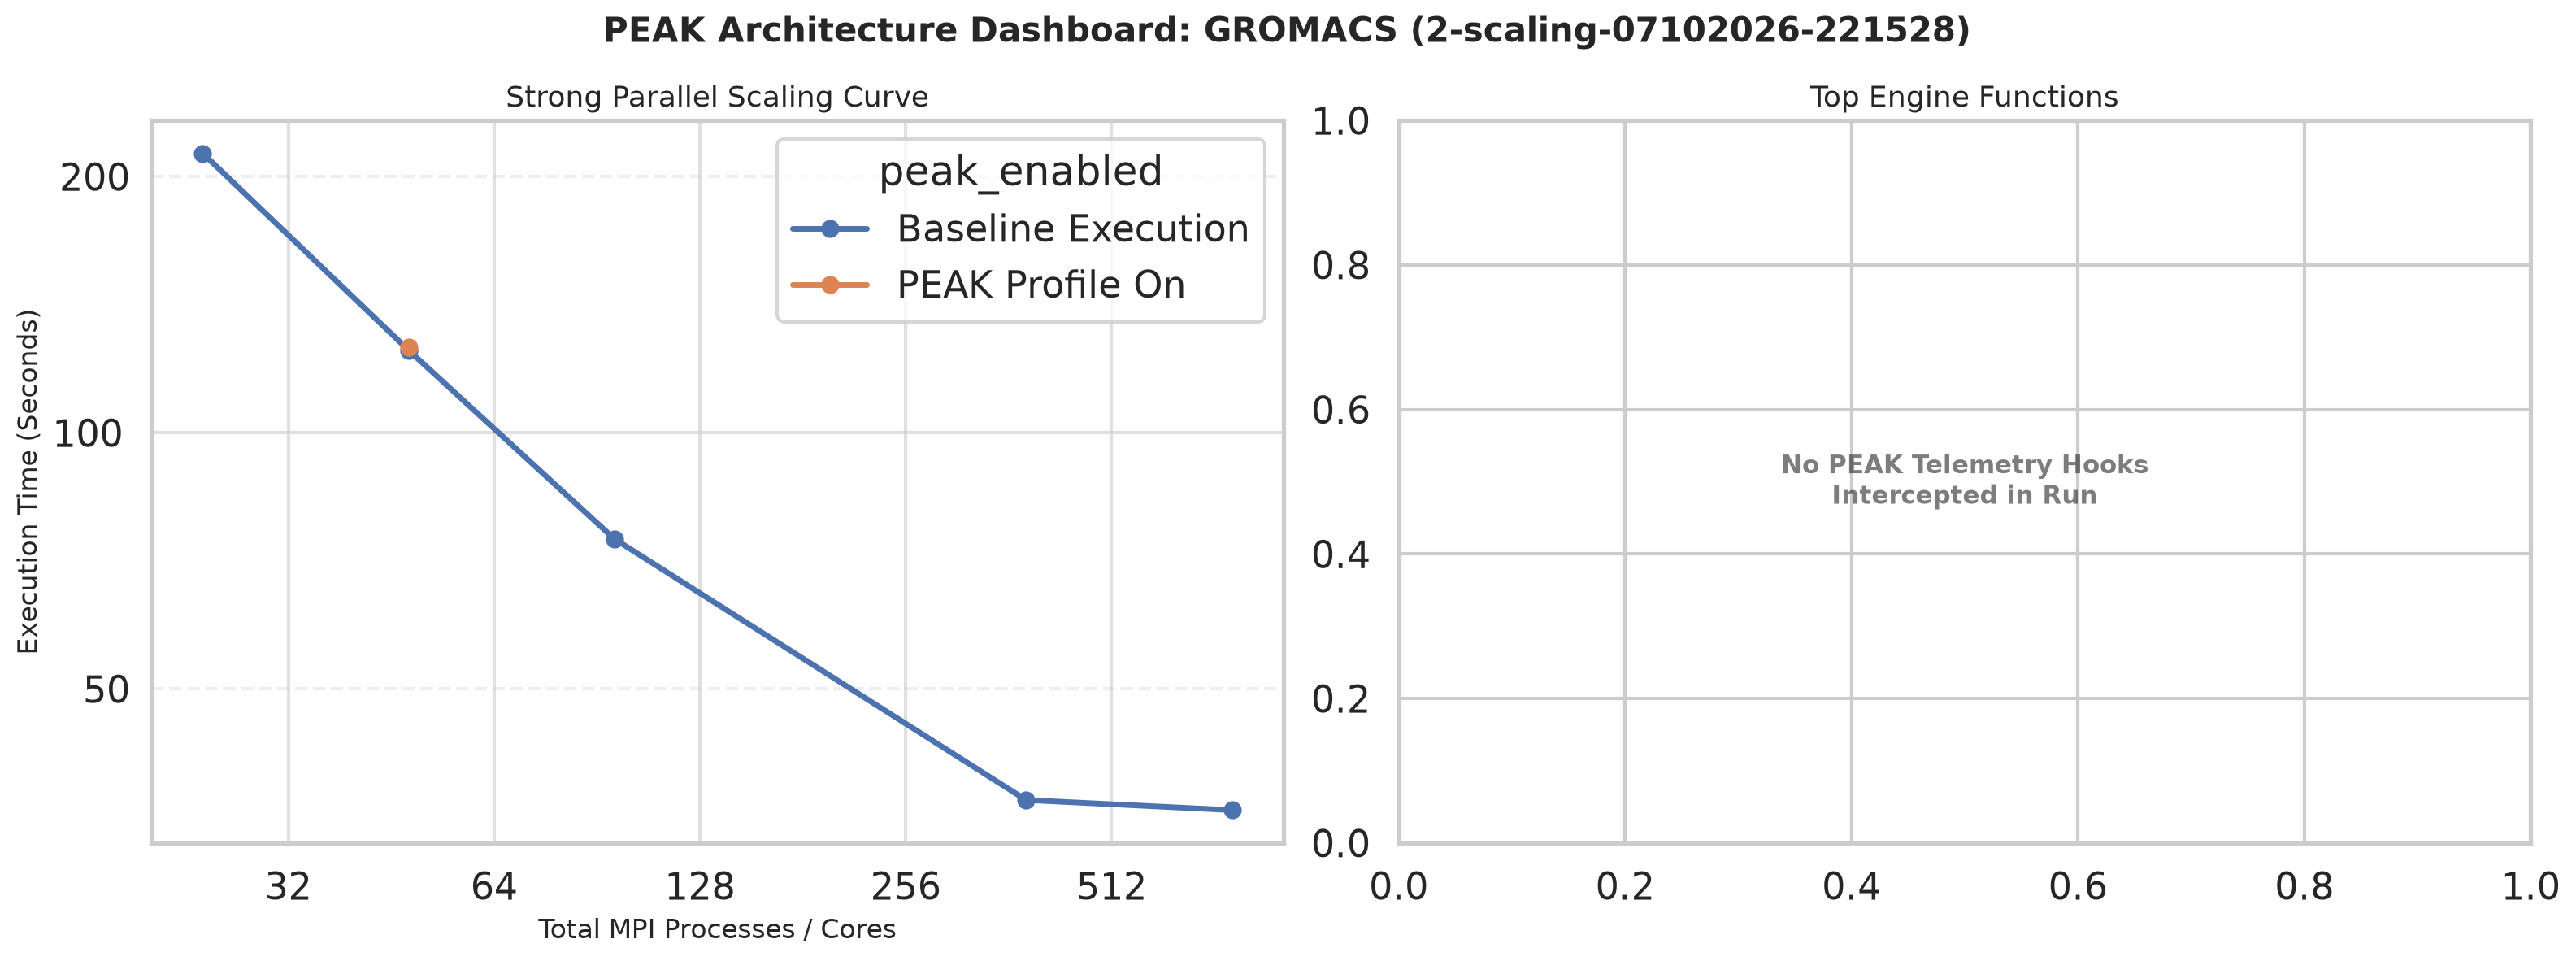
\includegraphics[keepaspectratio]{../plots/gromacs_2-scaling-07102026-221528_dashboard.png}}
\caption{plot}
\end{figure}

\subparagraph{Takeaway}\label{takeaway-4}

\begin{itemize}
\tightlist
\item
  GROMACS seemingly takes great advantage of scaling.
\end{itemize}

\subsubsection{Created another script to parse research data and create
graphs}\label{created-another-script-to-parse-research-data-and-create-graphs}

\subsection{What I Learned}\label{what-i-learned}

\begin{itemize}
\tightlist
\item
  Creating input files
\item
  Working with QE, DFTB+, LAMMPS, and GROMACS
\item
  Interpreting profiling data
\end{itemize}

\subsection{Questions / Concerns}\label{questions-concerns}

\begin{itemize}
\tightlist
\item
  For cases where PEAK does not get any hits for BLAS, LAPACK, and FFTW.
  Is there anything else you would want me to do or try?

  \begin{itemize}
  \tightlist
  \item
    From what I've looked into, it may be due to the way these programs
    were compiled as for why I'm getting no hits.
  \end{itemize}
\item
  For DFTB+, I am using the spinlock case for testing. Is there a
  different test case I could use?
\end{itemize}

\end{document}
